\documentclass[UTF8]{ctexart}

%固定图片位置
\usepackage{float}

%插入超链接
\usepackage{url}

\usepackage{tikz,mathpazo}
\usetikzlibrary{shapes.geometric, arrows}
\usetikzlibrary{calc}

%\usepackage[affil-it]{authblk}

\usepackage{listings}
%插入代码的配置
\definecolor{CPPLight}  {HTML} {686868}
\definecolor{CPPSteel}  {HTML} {888888}
\definecolor{CPPDark}   {HTML} {262626}
\definecolor{CPPBlue}   {HTML} {4172A3}
\definecolor{CPPGreen}  {HTML} {487818}
\definecolor{CPPBrown}  {HTML} {A07040}
\definecolor{CPPRed}    {HTML} {AD4D3A}
\definecolor{CPPViolet} {HTML} {7040A0}
\definecolor{CPPGray}  {HTML} {B8B8B8}
\lstset{
	language=Matlab,                                     % 设置语言
    columns=fixed,    
    breaklines = true,   
    basicstyle=\small ,
    numbers=left,                                        % 在左侧显示行号
    %frame=none,                                          % 不显示背景边框
    backgroundcolor=\color[RGB]{245,245,244},            % 设定背景颜色
    keywordstyle=\color[RGB]{40,40,255}\bfseries,                 % 设定关键字颜色
    %commentstyle=\color{red!10!green!70}\textit,    % 设置代码注释的颜色
    numberstyle=\tiny\color{darkgray},           % 设定行号格式
    commentstyle=\it\color[RGB]{0,96,96},                % 设置代码注释的格式
    stringstyle=\rmfamily\slshape\color[RGB]{128,0,0},   % 设置字符串格式
    showstringspaces=false,                              % 不显示字符串中的空格                           
    %morekeywords={True,alignas,continute,friend,register,true,alignof,decltype,goto,
    %reinterpret_cast,try,asm,defult,if,return,typedef,auto,delete,inline,short,
    %typeid,bool,do,int,signed,typename,break,double,long,sizeof,union,case,
    %dynamic_cast,mutable,static,unsigned,catch,else,namespace,static_assert,using,
    %char,enum,new,static_cast,virtual,char16_t,char32_t,explict,noexcept,struct,
    %void,export,nullptr,switch,volatile,class,extern,operator,template,wchar_t,
    %const,false,private,this,while,constexpr,float,protected,thread_local,
    %const_cast,for,public,throw,std,rand},
    emph={access,and,break,class,continue,def,del,elif ,else,%
	except,exec,finally,for,from,global,if,import,in,i s,%
	lambda,not,or,pass,print,raise,return,try,while, imshow, subplot, figure,%
    log, fft2, fftshift, abs, size, rgb2gray, imread},
    emphstyle=\color{CPPViolet}\bfseries, 
    emph={[2]True, False, None, self},
	emphstyle=[2]\color{green},
	emph={[3]from, import, as},
	emphstyle=[3]\color{blue},
	upquote=true,
	morecomment=[s]{"""}{"""},
    morecomment=[s]{\%}{},
	%commentstyle=\color{orange}\slshape,
    commentstyle=\color{red!10!green!70}\textit,    % 设置代码注释的颜色
	emph={[4]1, 2, 3, 4, 5, 6, 7, 8, 9, 0},
	emphstyle=[4]\color{red},
	emph={[5]numpy, np, plt},
	emphstyle=[5]\color{red},
	literate=*{:}{{\textcolor{blue}:}}{1}%
	{=}{{\textcolor{blue}=}}{1}%
	{-}{{\textcolor{blue}-}}{1}%
	{+}{{\textcolor{blue}+}}{1}%
	{*}{{\textcolor{blue}*}}{1}%
	{!}{{\textcolor{blue}!}}{1}%
	{(}{{\textcolor{blue}(}}{1}%
	{)}{{\textcolor{blue})}}{1}%
	{[}{{\textcolor{blue}[}}{1}%
	{]}{{\textcolor{blue}]}}{1}%
	{<}{{\textcolor{blue}<}}{1}%
	{>}{{\textcolor{blue}>}}{1},%
    %{\%}{{\textcolor{green}\%}}{1},%
	framexleftmargin=0.1mm, framextopmargin=0.1mm, frame=shadowbox, rulesepcolor=\color{black},
}



\usepackage{geometry}
\geometry{left=2cm, right=2cm, top=1.2cm, bottom=1.2cm}

%得到引用的标题内容
\usepackage{nameref} 

%添加首行缩进,两个字符
\usepackage{indentfirst}
\setlength{\parindent}{2em}

%多行公式一个编号
\usepackage{amsmath}

%文献引用,标准类型为plain
%\usepackage[hyperref=true,backend=biber,sorting=none,backref=true]{biblatex}
%\addbibresource{ref.bib}
\bibliographystyle{plain}
\usepackage{cite}

\pagestyle{plain}

%跨页表格
\usepackage{multirow}
\usepackage{longtable,booktabs}
\usepackage{supertabular}
\usepackage{makecell}

%调整itemize等的间距
\usepackage{enumitem}


\usepackage{graphicx}
\usepackage{subfigure}

%超链接
\usepackage[linkcolor=yellow,citecolor=red,backref=page,hyperfootnotes=true]{hyperref}
\hypersetup{
bookmarks=true,
colorlinks=true,
linkcolor=black
}
\usepackage{tabularx} %This package must be placed after package {hyperref}, otherwise footnote marks are NOT treated as hyperlinks.


%引入了一些改进的数学环境,如align
\usepackage{amsmath}

\title{数字图像处理报告五:频域知识与$CNN$的结合}
\author{姓名:鲁国锐 \protect\newline
\and 学号:17020021031 \\
\and 专业:电子信息科学与技术}
\date{2020年4月8日}

\begin{document}
	\maketitle
	\renewcommand{\contentsname}{目录}
	\renewcommand{\listfigurename}{插图目录}
	\renewcommand{\listtablename}{表格目录}
	\renewcommand{\refname}{参考文献}
	\renewcommand{\abstractname}{摘要}
	\renewcommand{\indexname}{索引}
	\renewcommand{\tablename}{表}
	\renewcommand{\figurename}{图}
	
	
	
	\tableofcontents
	\newpage
	
	\hypersetup{
	bookmarks=true,
	colorlinks=true,
	linkcolor=red,
	urlcolor=blue
	}
	\section{题目描述}
	\indent 试探讨如何将频率域知识用于卷积神经网络(可以从网上查阅相关资料)

			
%			\begin{figure}[H]
%				\centering 
%				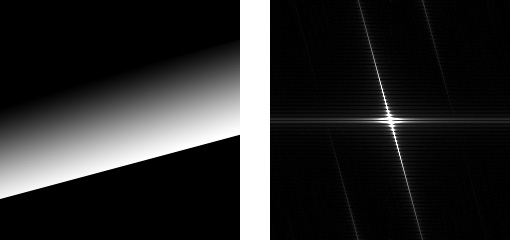
\includegraphics[scale=0.4]{org_img.png} 
%				\caption{原图及其傅里叶变换} 
%				\label{problem_img}
%			\end{figure}
		


	
	\section{问题背景}\label{background}
        \indent 在计算机视觉领域,深度神经网络已经得到相当广泛的应用,并已经在诸多方向上取得了非凡的成果。然而,现存的神经网络主要实行的是空间域的操作,且所处理图像的尺寸大小必须是固定的\cite{xu2020learning};而在现实生活中获得的图像尺寸一般是多样的,同时其尺寸往往也大于神经网络规定的输入尺寸。另外,大尺寸图像还会使得计算成本和片间通信带宽大大增加\cite{xu2020learning}。所以,基于可操作性的需要,图像通常都要被调整大小(下采样)以适应神经网络和降低计算成本及通信带宽\cite{xu2020learning}。
        
        \indent 但下采样又会带来新的问题。当图片尺寸被缩小后,分辨率降低,使得一些重要的信息被丢失\cite{xu2020learning},从而导致最终的结果不尽人意。例如,在人脸识别任务中,卷积神经网络($CNN$)对低分辨率图像识别的准确度要明显低于高分辨率图像\cite{huang2017wavelet}。
        
        \indent 在这种情况下,将频域中的信息作为输入交给神经网络可以有效减少下采样带来的信息损失\cite{xu2020learning}。除此之外,还可以用$CNN$对小波变换的系数进行预测,以此来构建超分辨率图像\cite{huang2017wavelet}。
    
    \section{方法简述}\label{solution}
    
        \subsection{将频域知识用于图像预处理}
            \indent \cite{xu2020learning}中提出了一种学习频域特征的通用方法,能够在减少计算量和通信带宽的同时尽可能多地保留信息,从而提高在分类、识别任务中的准确率。该方法大体分成两个部分:一个是提取频域特征的数据预处理方法,主要用来提升对图像信息的保留程度,增加分类、识别任务的准确度;另一个是对数据进行剪枝的方法,主要用于减少计算量和片间通信带宽。这里主要介绍前者。
            
            \indent 该预处理方法大致分为如下几步:
            
    			\begin{enumerate}[leftmargin=50pt]
    				\item 遵循图像预处理和数据增强的步骤,对其进行大小调整,裁剪和旋转;
    				\item 将图像转换到$YCbCr$色彩空间,再将图像转换到频域——这里用的是二维余弦变换($DCT$);
    				\item 将相同频率的二维$DCT$系数组合成一个通道,构成一个三维的$DCT$图像块;
    				\item 选择对结果影响最大的频率通道子集;
    				\item 将于$YCrCb$色彩空间中选出的通道连接在一起,形成一个张量;
                    \item 用从训练集中算出的均值和方差,来对每一个频率通道进行归一化。
    			\end{enumerate}
            
            \indent 操作流程也可见图\ref{pre-processing}。
            
            \indent 这种方法的好处在于,可以通过增加特征映射的通道数来缩短它的长和宽,同时还能保证总的点数不变,即将一张$H \times W \times C$的图转换成一张$ \frac{H}{M} \times \frac{W}{N} \times (C \times M \times N ) $的频域特征映射,从而维持着与输入图像相同的数据量。相应的,频域特征映射也可以跳过传统$CNN$的输入层;然后调整下一层的维度,使其能够直接接收频域特征映射。这样可以使对传统$CNN$结构的调整尽可能小。
            
            \indent \cite{xu2020learning}中的后续章节,证明了特征映射中的大部分频率通道可以被剔除而不会影响神经网络的准确度,同时也提出了相应的实现方法:基于学习的频率通道选择和静态频率通道选择。时间紧迫,这里不对其进一步阐述。
            
            \indent 另外,该论文也证明了卷积神经网络对低频通道更加敏感,这一点与人类视觉系统($HVS$)相似。这里同样不多做阐述。
    			
    			\begin{figure}[htbp]
    				\centering 
         			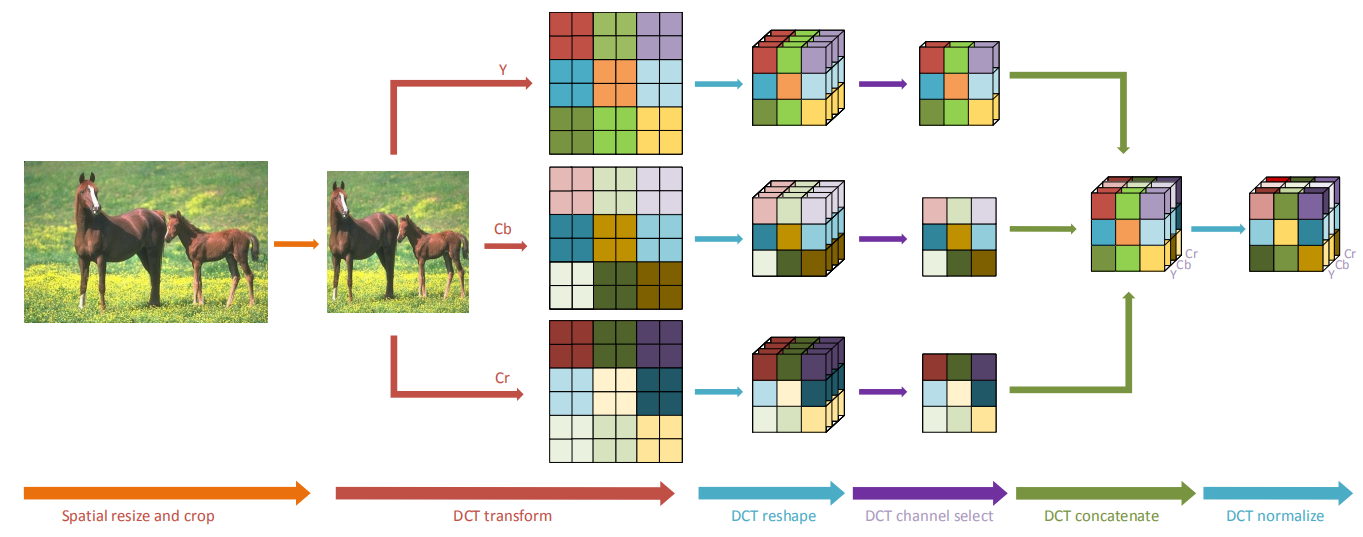
\includegraphics[scale=0.5]{pre-processing.png} 
    				\caption{预处理流程示意图} 
    				\label{pre-processing}
    			\end{figure}
        \subsection{用$CNN$预测小波变换系数}
            
            \indent \cite{huang2017wavelet}中提出了另一个思路:用卷积神经网络来预测图像的小波变换系数。这篇文章的作者们假设:只要一幅图像的小波变换系数能被准确地预估出来,就能根据一张低分辨率图像生成一张带有丰富纹理细节和全局拓扑结构信息的高分辨率图像。更进一步地说,强调高频小波系数有助于复现纹理细节;而加强对低频小波系数重建的约束则可以加强全局拓扑信息的一致性。因此,如何生成高分辨率图像这一问题就归结为了如何准确预测小波系数的问题。
            
            \indent 为了最大限度地发挥小波变换的优势,作者专门为其针对人脸识别这一任务设计了一个卷积神经网络结构。该网络结构又由三个子网络构成:
            
    			\begin{enumerate}[leftmargin=50pt]
    				\item 嵌入网络($embedding\ net$):输入一张低分辨率图像,输出一组特征映射;
    				\item 小波预测网络($wavelet\ prediction\ net$):它由一系列平行独立的子网组成,其中每一个子网的目的是用嵌入网络输出的特征映射来学习一个特定的小波系数;
                    \item 重建网络($reconstruction\ net$):由给定的小波系数恢复出一张高分辨率的图片。
    			\end{enumerate}
                
            \indent 由于时间紧张,没有时间再去深入学习小波变换,故对该论文的基本思想就只能介绍到这里。
            
%        \nocite{digit_image_Gonzalez}
%        \nocite{signal_and_system}
%        \nocite{discrete-time_signal_processing}



		

            


%			\indent 采取\ref{数字相机成像原理}节的方式,我们也可以把线性扫描相机的原理概括为以下$3$个步骤:
%			\begin{enumerate}[leftmargin=50pt]
%				\item 由条带传感器成像,给出一幅图像一行(或一列)的像素值;
%				\item 沿垂直于传感器带的方向移动一小段距离;
%				\item 重复步骤$1$和步骤$2$,直至整幅图像全部成像完毕。
%			\end{enumerate}

%		\begin{enumerate}[leftmargin=50pt]
%			\item 所成图像在垂直方向上的大小不受限制;
%			\item 能够通过提高扫描频率达到非常高的分辨率;
%			\item 使用起来灵活方便等
%		\end{enumerate}
		
%	\section{实验验证}
%        \subsection{实验思想}
%            \indent 从前面的分析可以看出,频谱图上的谱线与空间域中像素变化的方向及剧烈程度有关。从这个角度出发,如果把空间域图像转一个角度,频谱图中的谱线相应地也应该旋转相同的角度。我们将在之后的两个小节中对这个猜想进行验证。
%        \subsection{实验代码}
%            	\begin{lstlisting}[language=Matlab,caption={实验代码},label={broadcast.cpp}]
%% reference: https://blog.csdn.net/jiugedexiaodi/article/details/79705308
%
%
%
%img = imread('C:\Users\Asus-\Desktop\数字图像\report\04\rotate45.png');
%img = rgb2gray(img);
%
%% 将图像的数据格式转换为double型的,此时图像的数值范围由原来的[0,255],
%% 变成了[0,1],其实不进行转换的话,也可以进行傅里叶变换,
%% 只是傅里叶变换后的图像会有所不同
%img=im2double(img);
%
%% size(img)
%
%F = fft2(img);
%F = fftshift(F);
%F = abs(F);
%
%% 傅里叶变换后模值差异非常大,低频直流远远大于高频
%% 不加这一句变换后的结果只能看到中间有一个亮点
%T = log(1+F);
%figure(1)
%subplot(1, 2, 1)
%imshow(img)
%subplot(1, 2, 2)
%% 后面的[],表示对图像做了一个类似于归一化的操作,
%% 防止傅里叶变换后模值差异太大
%imshow(T, [])
%            	\end{lstlisting}
                

        
%            \begin{figure}[htbp]
%            	\centering 
%                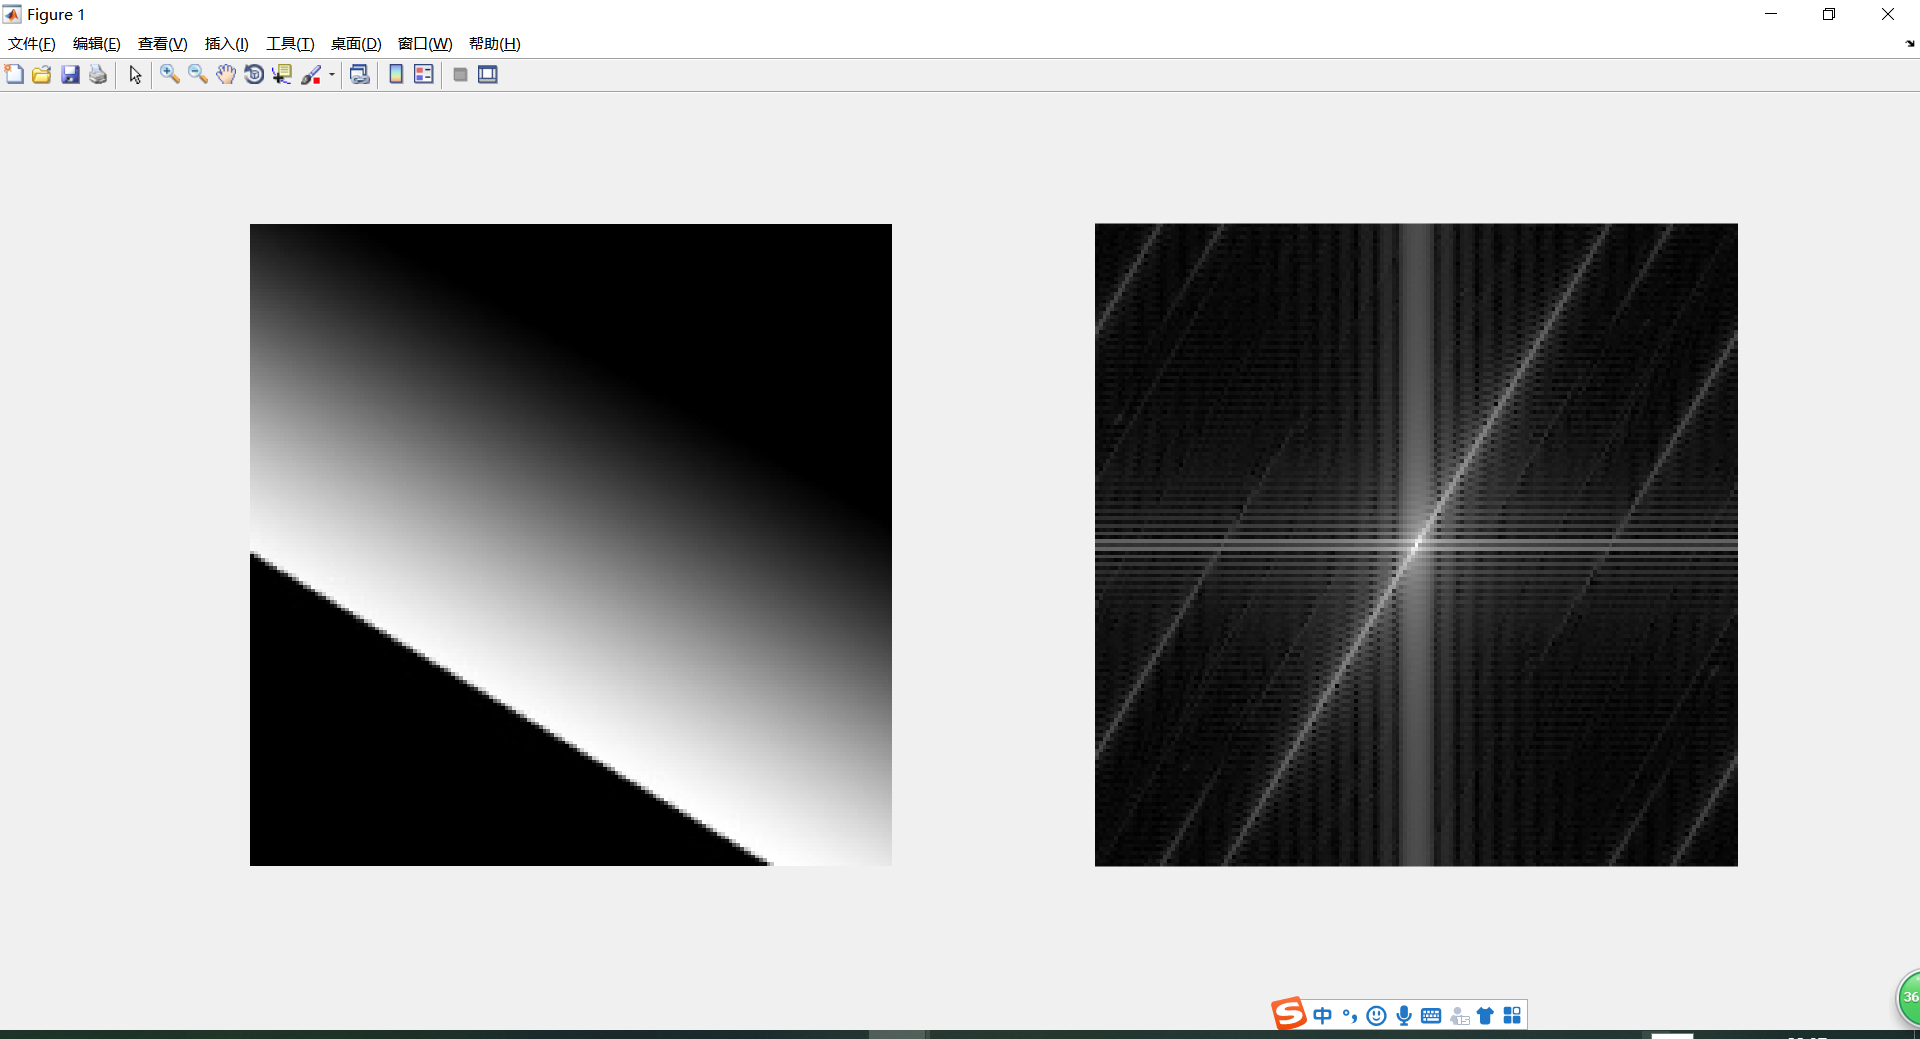
\includegraphics[scale=0.4]{result.png} 
%            	\caption{实验结果} 
%            	\label{result}
%            \end{figure}

            


	\section{总结}
		\indent 在本次报告中介绍了\cite{huang2017wavelet}和\cite{xu2020learning}两篇论文。由于水平有限,再加上时间紧迫,关于这两篇文章还有很多问题没有解决,如:为何要先将原图转换到$YCbCr$色彩空间;如何把相同频率的小波系数组合成一个通道,同时还能保证整个特征映射在各频率分量上的通道数一致等。
%			\begin{figure}[H]
%				\centering 
%				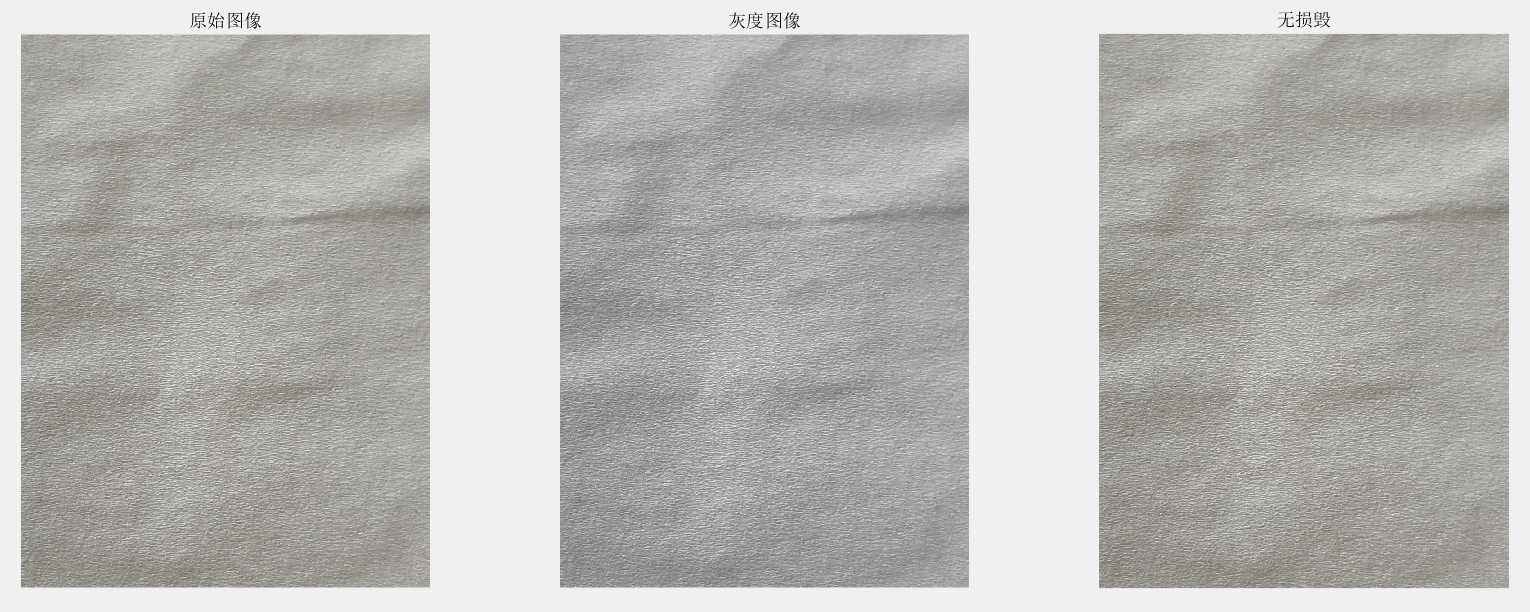
\includegraphics[scale=0.4]{res4.png} 
%				\caption{结果4} 
%				\label{res4}
%			\end{figure}
		

		
%			\begin{figure}[H]
%				\centering 
%				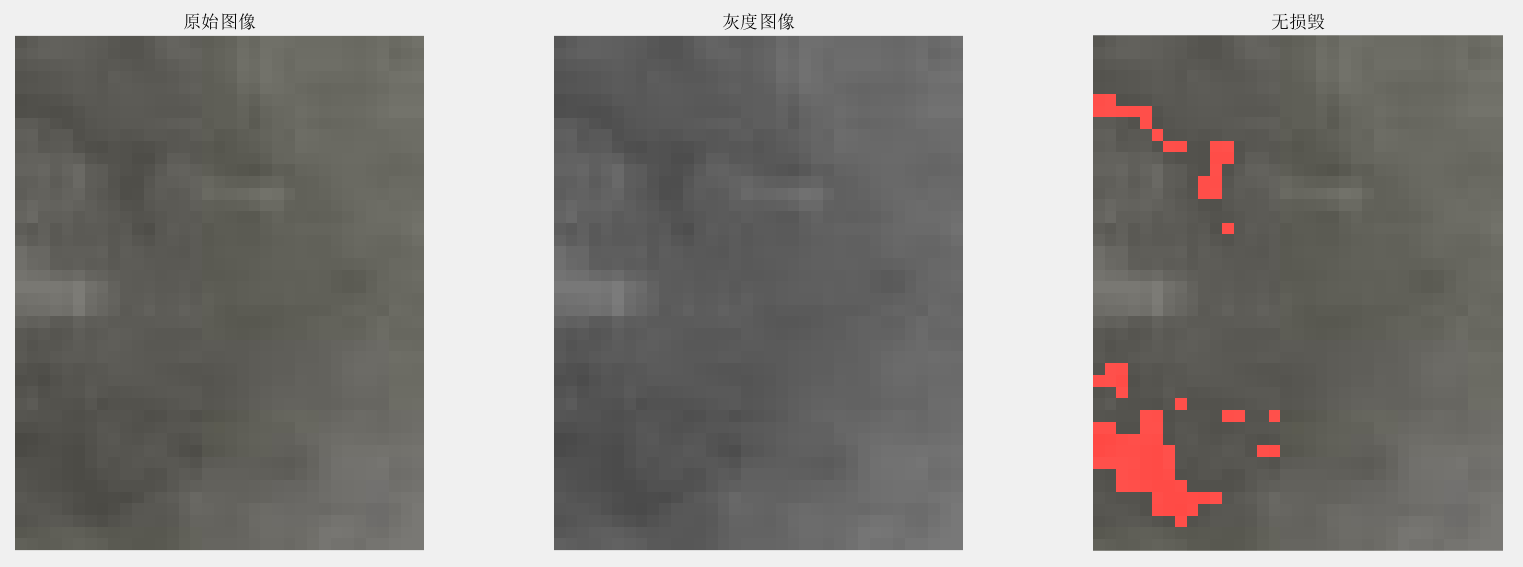
\includegraphics[scale=0.4]{res6.png} 
%				\caption{结果6(截取自结果5的阴影部分)} 
%				\label{res6}
%			\end{figure}
	
	
% 中文文献多个作者用中文逗号“,”连接
%\bibliography{ref.bib}
%\bibliographystyle{abbrv}
\bibliography{ref.bib}


\end{document}